%%%% utfpr-ic-report.tex, 2021/09/21
%%%% Copyright (C) 2017-2021 Luiz E. M. Lima (luizeduardomlima@gmail.com)
%%

%% Detecção e aviso sobre comandos obsoletos
% \RequirePackage[l2tabu, orthodox]{nag}

%% Classe de documento
\documentclass[%% Opções: (^) padrão; (>) para pacotes
  a4paper,%% Tamanho de papel: a4paper, letterpaper (^), etc.
  12pt,%% Tamanho de fonte: 10pt (^), 11pt, 12pt, etc.
  %fleqn,%% Alinhamento de equações à esquerda (centralizado por padrão)
  % draft,%% Aparência do documento (>): draft ou final (^)
  english,%% Idioma secundário (penúltimo) (>)
  brazilian,%% Idioma primário (último) (>)
]{article}

%% Pacotes utilizados
\usepackage[%% Opções: (^) padrão
   %DocLic  = CC,%% Licença do documento: CC (Creative Commons) ou None (^)
   %CCLic   = BY-SA-ND,%% Licença CC: BY (^), BY-SA, BY-ND, BY-NC, BY-NC-SA ou BY-NC-ND
   Link    = TextColor,%% Cor de hyperlinks: DarkBlue (^) ou TextColor
   ABNTCit = AAY,%% Citação ABNT: AAY (NOME, ANO), NRB (1) ou NSB [1] (^)
   BibURL  = Icon,%% Links de URLs nas referências: Icon ou Text (^)
]{utfpr-ic-report}

\Title{Aplicativo para gestão de manutenção industrial}

\Student{
  Name      = {
    André Luiz da Silva Junior\\
    Bruno Soares Dias\\
    Gabriel Zuin Jarduli\\}%
 }
  
\Campus{Cornélio Procópio}
 \Date{2022}

%% Início do documento
\begin{document}

\section{Introdução}%
As indústrias têm uma grande dependência de seu maquinário, se o mesmo ficar muito tempo parado a empresa tem menos produtividade. Para se evitar o mau funcionamento e a parada da fábrica, ao longo do tempo vem se criando vários métodos para corrigir e prevenir estes problemas, atualmente tem-se três formas de aplicação: corretiva, preventiva e preditiva. De maneira geral as logísticas de manutenção buscam otimizar o desempenho e a eficiência da máquina, a manutenção corretiva é voltada no conserto de peças com mau funcionamento ou quebradas onde se planeja ou não a manutenção do maquinário, já com mais planejamento a preventiva faz manutenções periodicamente visando o tempo de vida das peças, junto ao surgimento da indústria 4.0 a manutenção preditiva permite que se instale sensores nos mecanismos onde se consegue captar anomalias que indicam que há algo errado e possibilita o planejamento da manutenção antes que a máquina, de fato, apresente problemas [01]. O maquinario industrial é composto por maquinas eletronica, eletromecanica, analogica ou pinelmatica, podedo atuar em varios setores da industria sendo agricula, construcao, saude, mineracao, producao (carro, materiais,etc ... ).

%Buscar uma area para aplicar

\section{Objetivos}%
Este projeto tem como objetivo auxiliar qualquer empresa que atue em area industrial que esteja com problemas de questões logísticas em reparação e manutenção de máquinas. Tendo a total liberdade da equipe de manutenção acessar e alimentar o sistema de qualquer lugar da fábrica e  também dos líderes dos outros setores conseguirem abrir solicitações sem a necessidade de ir até o computador.

%detalhar em topicos

\begin{figure}[!htb]

\includegraphics[width = 0.95\linewidth]{Figures/1.png}
\caption{Diagrama}%
\end{figure}

O aplicativo abordará 
\begin{itemize}
    \item Agenda para auxiliar os funcionários
    \item Solicitação de serviço
    \item equipamentos/ferramentas a serem utilizadas
    \item uma dashboard que mostra o serviço contendo:
    \begin{itemize}
    \item custo previsto
    \item equipamento
    \item prioridade 
    \item data de inicio/termino
    \item preço final da manutenção
    \item funcionários na manutenção
    \end{itemize}    
\end{itemize}
    

\section{Justificativa}%
Informatizar a gestão da manutenção tem suas vantagens, como por exemplo, simplificar o cotidiano dos funcionários e facilitar a análise de dados, por estarem organizados e presentes em um só lugar. Mesmo assim, muitas empresas de pequeno ou médio porte ainda não utilizam da tecnologia para obter os benefícios que ela é capaz de oferecer. Portanto, pelo que já foi descrito e pela dificuldade em se obter um produto bom que atenda as necessidades básicas da manutenção de forma gratuita ou de baixo custo, faremos um aplicativo que ajude essa parte da indústria que ainda está no vazio tecnológico, queremos ajudar a entrar na industria 4.0, podendo ser das areas agricula, construcao, saude, mineracao, producao.

\subsection{Produtos Similares}
\begin{enumerate}
    \item Keepfy
    \item Fracttal
    \item Infraspeak
    \item Fluix
\end{enumerate}

%levantar potenciais usuarios
%falar das empresas com produtos similares econtextualizar quais as inovações do serviço/produto proposto no trabalho, como diferenciais que justifiquem o seu desenvolvimento (preço por exemplo, tecnologia nacional, etc.)

\section{Materiais e Métodos}%

%- Materiais: conjunto de dados que eventualmente sejam importantes para a projeto, como um dataset que será utilizado;
%- Métodos: quais ferramentas de desenvolvimento, tecnologias, hardware, banco de dados, etc. que serão empregadas, incluindo a respectiva descrição e indicando a funcionalidade que terá no desenvolvimento do projeto.


\subsection{Materiais:}%
Para criação do aplicativo, uma fábrica de compressores do interior de São Paulo será utilizada como referência, as planilhas de gestão de manutenções preventivas e corretivas e o e-mail de solicitação de serviço serão analisados para que o produto ofereça as mesmas possibilidades que se tem no modelo atual, tanto na modelagem dos dados quanto no design.

\subsection{Métodos:}%
O front-end será feito com a linguagem TypeScript utilizando o framework React Native que possibilita uma versatilidade no desenvolvimento sendo compatível com iOS e Android.
O Google Firebase será a ferramenta utilizada como banco de dados(substituindo o MySQL definido anteriormente). 
Para organizar a produtividade do grupo, será utilizado o Trello para gerenciar as tarefas a serem feitas, GitHub para compartilhamento e versionamento do aplicativo. 



%- Incluam referências bibliográficas de toda a fonte de informação qe usarem, referenciando o texto que usarem afirmações ou dados dessas fontes.
%- Tentem especificar melhor e atualizar o cronograma. É importante que fique clara a relação entre as atividades do cronograma e os objetivos e funcionalidades do projeto, para as tarefas previstas tentem identificar o responsável por cada tarefa.
%- Sei que iniciaram o projeto, ainda está em construção, por isso mesmo as indicações acima. Qualquer dúvida me digam. Como disse em aula, existe um bom potencial na ideia/projeto de vcs!



\section{Cronograma}%
A realização das atividades do projeto foi definida da seguinte forma:

\begin{figure}[!htb]
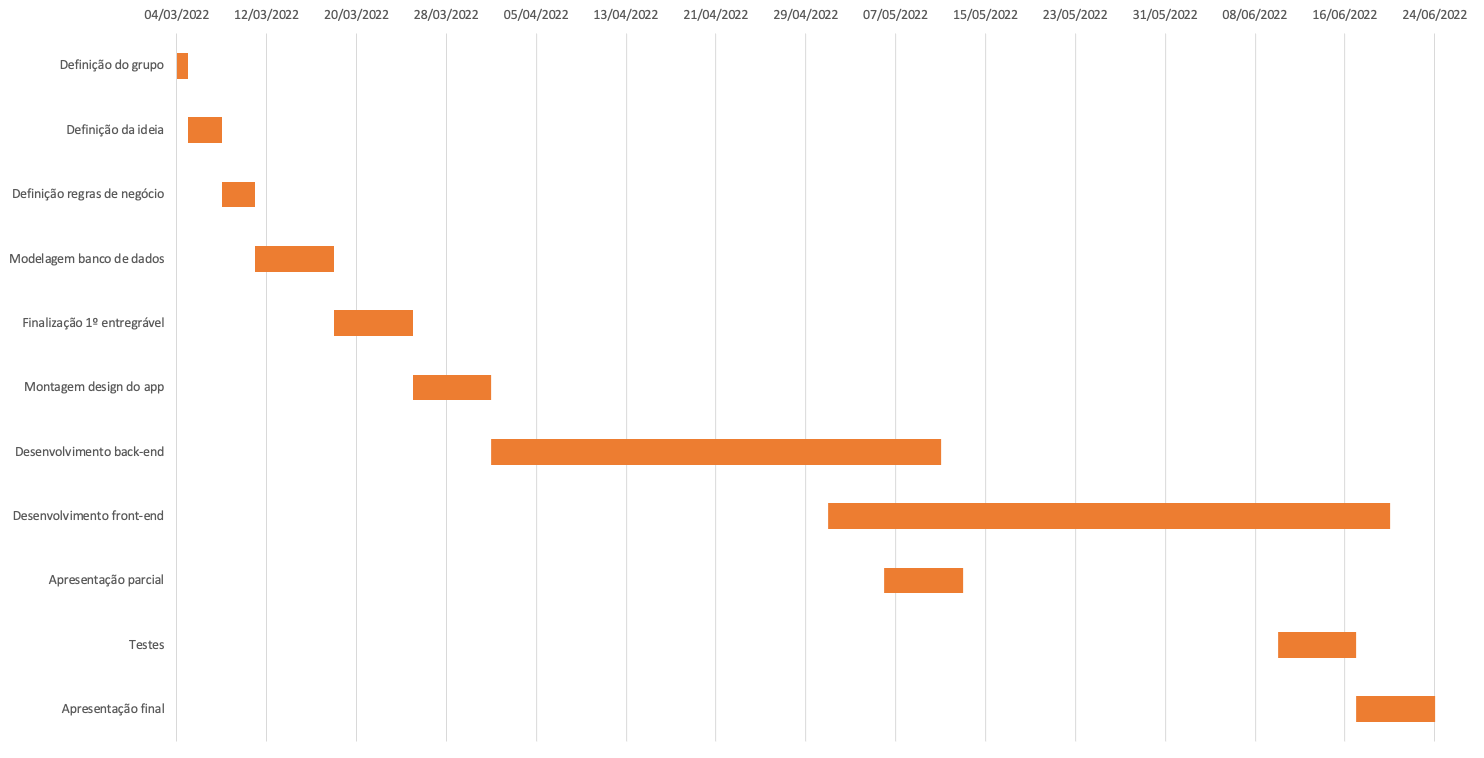
\includegraphics[width = 0.95\linewidth]{Figures/grafico.png}
\caption{Gráfico de tarefas}
\end{figure}
\begin{figure}[!htb]
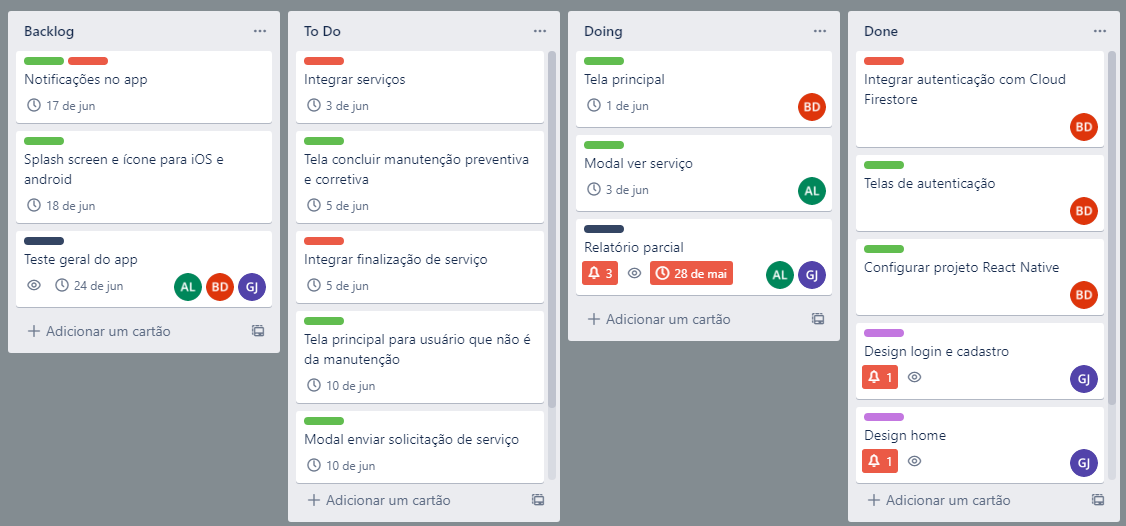
\includegraphics[width = 0.95\linewidth]{Figures/imagem.PNG}
\caption{Planejamento}
\end{figure}

\section{Referências}%
[01] A LOGÍSTICA NA MANUTENÇÃO: QUAIS OS TIPOS. \textbf{Portalic}, 2019. Disponível em: <http://www.portalic.com.br/blog/sua-industria/a-logistica-na-manutencao-quais-os-tipos/>. Acesso em: 10, março de 2022.\par
[02] GRÁFICO DE GANTT: O QUE É, COMO FUNCIONA E COMO MONTAR O SEU. \textbf{Nomus}, 2021. Disponível em: <https://www.nomus.com.br/blog-industrial/grafico-de-gantt/>. Acesso em: 13, março de 2022.
[03] LOGISTICS MANAGEMENT: \textit{Annual Maintenance Repair and Operations (MRO) Survey 2018: Spending on the rise}. Acesso em: 14 de março 2022.\par
[04] INFRASPEAK: Estatísticas de manutenção [2018-2021]: desafios, tendências e métricas. Disponível em: <https://blog.infraspeak.com/pt-br/estatisticas-de-manutencao/> Acesso em 14 de março de 2022.\par
[05]\textit{Predictive Maintenance 4.0 Beyond the hype: PdM 4.0 delivers results}. \textbf{PwC, Mainnovation}.Disponível em: <https://www.pwc.be/en/documents/20180926-pdm40-beyond-the-hype-report.pdf>. Acesso em 20 de março de 2022.

%% Fim do documento
\end{document}
